\chapter{Ausblick}

Sowohl durch den Industriepartner als auch durch das Team selbst kamen verschiedene Ideen für weitergehende Features auf. Aus Zeitgründen konnten leider nicht alle Ideen umgesetzt werden.

\section{'Workflow'}

Ein Wunsch der Industriepartner war es, den momentanen Arbeitsablauf abbilden zu können. Ein Beispiel ist, dass zuerst die 'unkritischen' Pakete auf den 'unkritischen' Systemen installiert werden müssen, bevor dort 'kritische' Pakete installiert werden können.

Dies wurde im 'Workflow'-Feature als Vorschlag präsentiert (Bild \ref{fig:ausblick:workflow}). Hier gibt es eine definierbare Reihenfolge von Arbeitsschritten, welche nacheinander durchgeführt werden müssen. Diese Arbeitsschritte könnten manuell festgelegt und bearbeitet sowie sortiert werden (Siehe Bild \ref{fig:ausblick:workflow_crud} für den Edit-Modus).


\xxx[ Workflow-Feature ]

\begin{figure}[H]
	\centering
	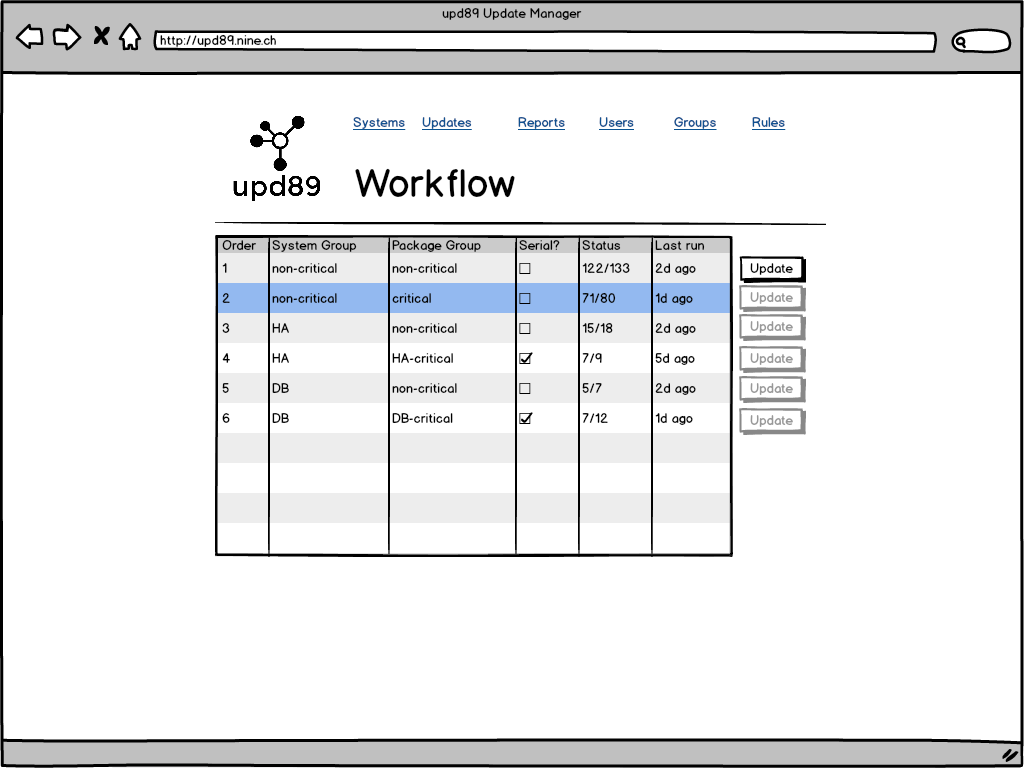
\includegraphics[width=\linewidth]{files/mockups/workflow}
	\caption{Konzept Workflow-Feature}
	\label{fig:ausblick:workflow}
\end{figure}

\begin{figure}[H]
	\centering
	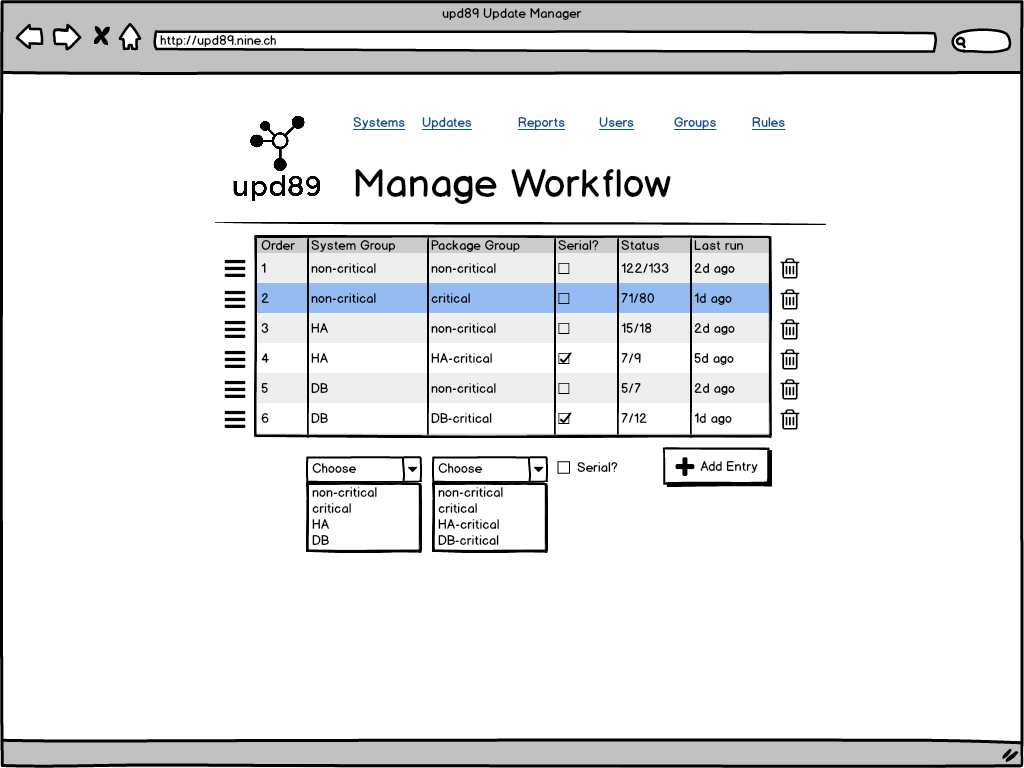
\includegraphics[width=\linewidth]{files/mockups/workflow_CRUD}
	\caption{Konzept Workflow-Feature bearbeiten}
	\label{fig:ausblick:workflow_crud}
\end{figure}

\xxx[ Separater API-Endpunkt für einfachere Registrierung, wie Puppet ]

\section{Dry-Run}

In \gls{apt} existiert das Feature 'dry-run', womit ein Updatevorgang simuliert\footnote{es werden keine Updates installiert, siehe auch \purl{http://linux.die.net/man/8/apt-get}} werden kann. Dies könnte auch als Feature im \gls{controlcenter} implementiert werden, indem vor dem Versenden eines Tasks zuerst eine Simulation durchgeführt werden könnte, um zu sehen, welche Pakete Abhängigkeiten nach sich ziehen oder fehlschlagen würden.

\section{Message-Queue}


\xxx[ Message-Queue, z.B. RabbitMQ ]

